\section{Data analysis}
\label{sec:analysis}

In this section we first perform an initial analysis of the data. We check their distributions and assess whether transformations should be performed for better expected results. Furthermore, we can get an initial idea of what variables will perform well by comparing the mean values for people with and without a Nobel Prize. This analysis is done using the R statistical software package.

Next, the logistic regression model is learned on the resulting dataset and evaluated using cross-validation. We experiment with excluding variables that are not relevant and balancing the number of positive and negative examples.

\subsection{Quality assessment}
\label{ssec:quality}

The merged dataset contains two variables that are \emph{fuzzy}: the number of likes on Facebook, which serves as a popularity measure, and the number of results for a specialised Google Scholar search, which serves as a productivity measure. Both might be prone to errors. Furthermore, some normalisation should be performed so that variables with a larger scale do not receive more weight in the final model. Since the university rankings are on a scale of $[0, 100]$ we will transform all variables to that scale.

\subsubsection{Popularity measure}
\label{sssec:popularity}
The popularity measure comes from gathering the number of likes on Facebook. Because this is done automatically and popular names might occur more than ones, we should check for outliers. A boxplot is shown in Figure~\ref{fig:popuInitialBox} and a density plot in Figure~\ref{fig:popuInitialDensity}. We can immediately see a problem: the outlier at 17 million deforms the distribution. It is the result for Einstein, however, and not an error in the data. Manual verification confirmed this for all seemingly high values. In order to solve this without having to remove any data, we perform a transformation using the natural logarithm. Logarithmic transformations are often used to normalise right-skewed distributions. The exact transformation is given by
\begin{equation}
\label{eq:logtransform}
t(x) = \begin{cases} ln(x), & \mbox{if } x \neq 0 \\ 0, & \mbox{if } x = 0 \end{cases}
\end{equation}
in order to correct $ln(0) = -\infty$. The same plots for the resulting distribution are given in Figures~\ref{fig:popuTransformedBox} and \ref{fig:popuTransformedDensity}. While still being far from normal, the outliers are now far less extreme. Next, the results are normalised by dividing by the maximal value and rescaled to $[0, 100]$.

In order to get an initial estimate whether it will be significant in the model, we can compare the mean value for winners and non-winners. Since there are sufficient examples, we may assume normality of sampling distributions and perform a standard two-sample $t$ test for unequal variances. The sample means are 
\begin{table}[H]
\centering
\begin{tabular}{c|c}
\textbf{\textsc{Nobel}} & \textbf{\textsc{Non-nobel}} \\ \hline
\rule{0pt}{4mm}23.05663&14.44544\\
\end{tabular}
\end{table}
Using R we find that the true means are not equal, which is what we hoped for the model.
\begin{figure*}
    \centering
    \begin{subfigure}[b]{0.4\textwidth}
        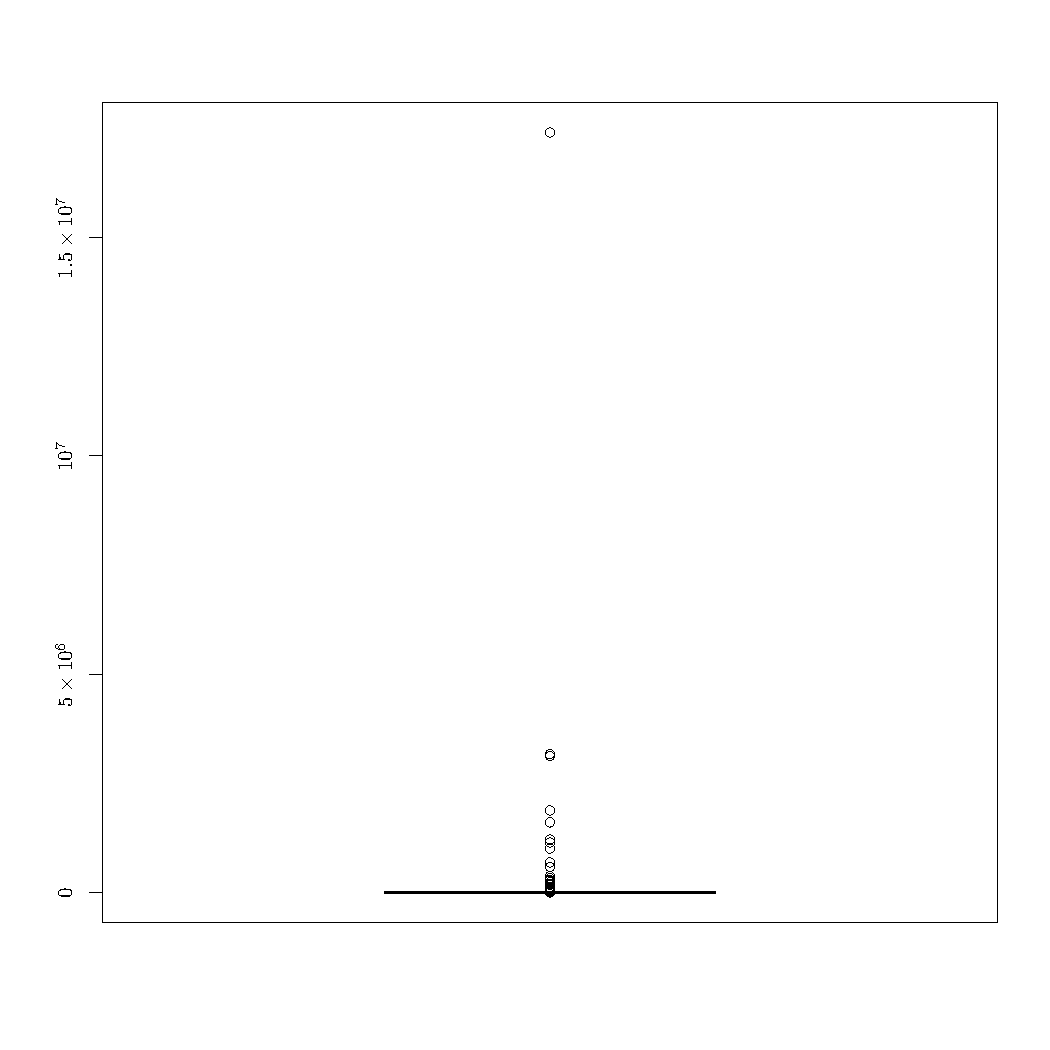
\includegraphics[width=\textwidth]{figures/popuInitialBox.pdf}
        \caption{Boxplot}
        \label{fig:popuInitialBox}
    \end{subfigure}
    ~
    \begin{subfigure}[b]{0.4\textwidth}
        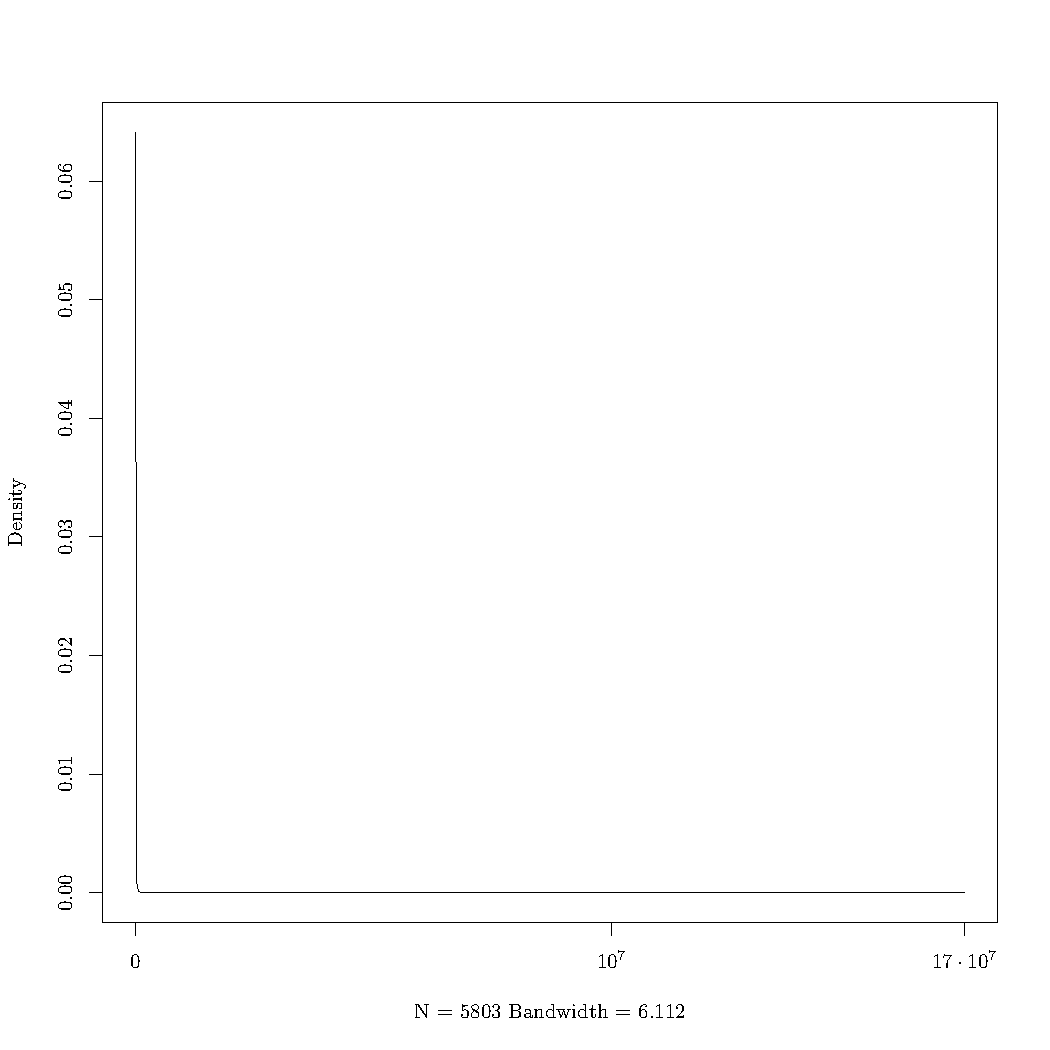
\includegraphics[width=\textwidth]{figures/popuInitialDensity}
        \caption{Density plot}
        \label{fig:popuInitialDensity}
    \end{subfigure}
    \caption{Distribution plots for raw popularity measure.}
\end{figure*}
\begin{figure*}
    \centering
    \begin{subfigure}[b]{0.4\textwidth}
        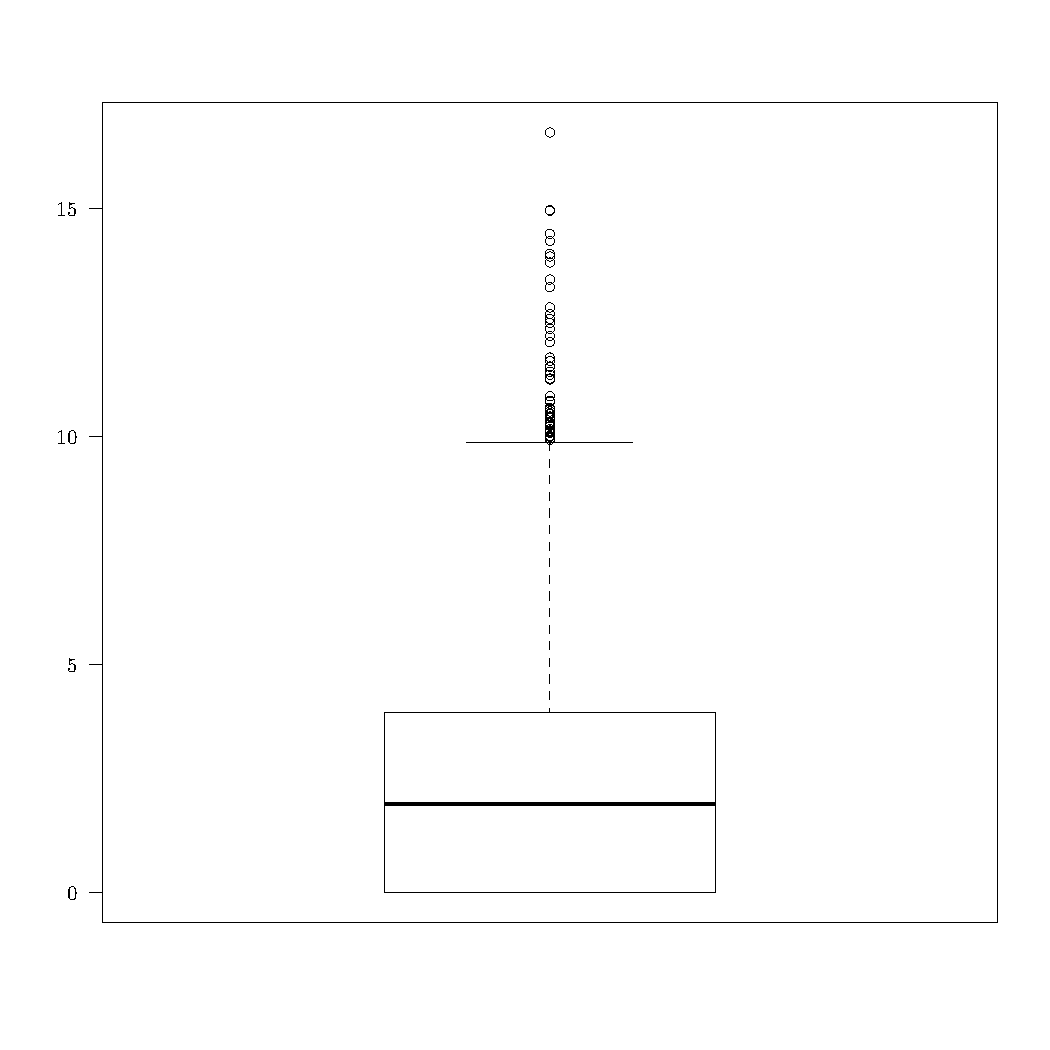
\includegraphics[width=\textwidth]{figures/popuTransformedBox}
        \caption{Boxplot}
        \label{fig:popuTransformedBox}
    \end{subfigure}
    ~
    \begin{subfigure}[b]{0.4\textwidth}
        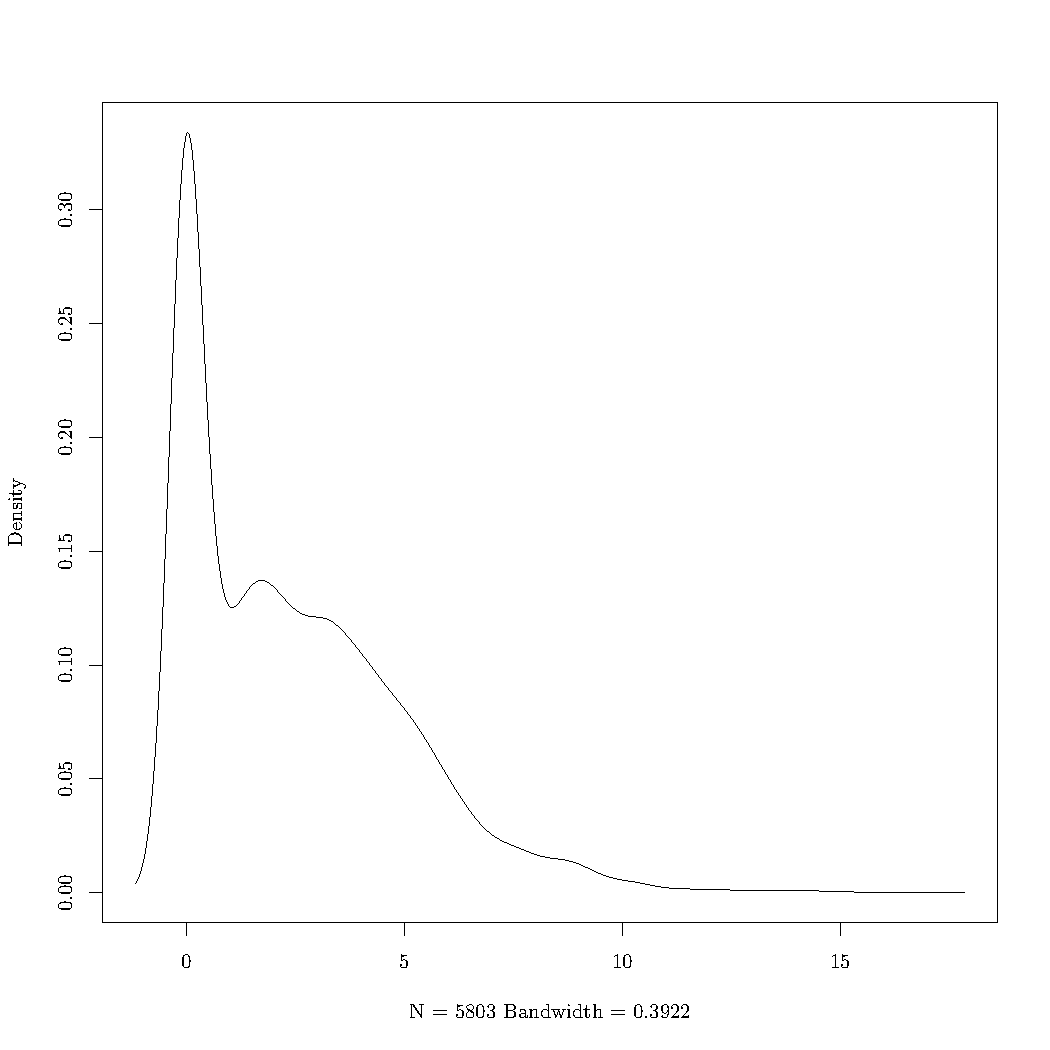
\includegraphics[width=\textwidth]{figures/popuTransformedDensity}
        \caption{Density plot}
        \label{fig:popuTransformedDensity}
    \end{subfigure}
    \caption{Distribution plots for transformed popularity measure.}
\end{figure*}

\subsubsection{Productivity measure}
\label{sssec:productivity}


\subsection{Learning a model}


\todo[inline]{Statistieken i.v.m training en research sets hier?}

\todo[inline]{figuren hier ter visualisatie data}

\todo[inline]{Sectie over difficulties (training data veel negatieve en weinig positieve examples, links die er niet zijn}